%% file: template.tex = LaTeX template for article-like report 
%% init: sometime 1993
%% last: Feb  8 2015  Rob Rutten  Deil
%% site: http://www.staff.science.uu.nl/~rutte101/rrweb/rjr-edu/manuals/student-report/

%% First read ``latex-bibtex-simple-manual.txt'' at
%% http://www.staff.science.uu.nl/~rutte101/Report_recipe.html

%% Start your report production by copying this file into your XXXX.tex.
%% Small changes to the header part will make it an A&A or ApJ manuscript.

%%%%%%%%%%%%%%%%%%%%%%%%%%%%%%%%%%%%%%%%%%%%%%%%%%%%%%%%%%%%%%%%%%%%%%%%%%%%
\documentclass{aa}   %% Astronomy & Astrophysics style class

\usepackage{graphicx,natbib,url,twoopt}
\usepackage[varg]{txfonts}           %% A&A font choice
\usepackage{hyperref}                %% for pdflatex
%%\usepackage[breaklinks]{hyperref}  %% for latex+dvips
%%\usepackage{breakurl}              %% for latex+dvips
\usepackage{pdfcomment}              %% for popup acronym meanings
\usepackage{acronym}                 %% for popup acronym meanings

\hypersetup{
  colorlinks=true,   %% links colored instead of frames
  urlcolor=blue,     %% external hyperlinks
  linkcolor=red,     %% internal latex links (eg Fig)
}

\bibpunct{(}{)}{;}{a}{}{,}    %% natbib cite format used by A&A and ApJ

\pagestyle{plain}   %% undo the fancy A&A pagestyle 

%% Add commands to add a note or link to a reference
\makeatletter
\newcommand{\bibnote}[2]{\@namedef{#1note}{#2}}
\newcommand{\biblink}[2]{\@namedef{#1link}{#2}}
\makeatother

%% Commands to make citations ADS clickers and to add such also to refs
%% May 2014: they give error stops ("Illegal parameter number ..."}
%%   for plain latex with TeX Live 2013; the ad-hoc fixes added below let
%%   latex continue instead of stop within these commands.
%%   Please let me know if you know a better fix!
%%   No such problem when using pdflatex.
\makeatletter
 \newcommandtwoopt{\citeads}[3][][]{%
   \nonstopmode%              %% fix to not stop at error message in latex
   \href{http://adsabs.harvard.edu/abs/#3}%
        {\def\hyper@linkstart##1##2{}%
         \let\hyper@linkend\@empty\citealp[#1][#2]{#3}}%   %% Rutten, 2000
   \biblink{#3}{\href{http://adsabs.harvard.edu/abs/#3}{ADS}}%
   \errorstopmode}            %% fix to resume stopping at error messages 
 \newcommandtwoopt{\citepads}[3][][]{%
   \nonstopmode%              %% fix to not stop at error message in latex
   \href{http://adsabs.harvard.edu/abs/#3}%
        {\def\hyper@linkstart##1##2{}%
         \let\hyper@linkend\@empty\citep[#1][#2]{#3}}%     %% (Rutten 2000)
   \biblink{#3}{\href{http://adsabs.harvard.edu/abs/#3}{ADS}}%
   \errorstopmode}            %% fix to resume stopping at error messages
 \newcommandtwoopt{\citetads}[3][][]{%
   \nonstopmode%              %% fix to not stop at error message in latex
   \href{http://adsabs.harvard.edu/abs/#3}%
        {\def\hyper@linkstart##1##2{}%
         \let\hyper@linkend\@empty\citet[#1][#2]{#3}}%     %% Rutten (2000)
   \biblink{#3}{\href{http://adsabs.harvard.edu/abs/#3}{ADS}}%
   \errorstopmode}            %% fix to resume stopping at error messages 
 \newcommandtwoopt{\citeyearads}[3][][]{%
   \nonstopmode%              %% fix to not stop at error message in latex
   \href{http://adsabs.harvard.edu/abs/#3}%
        {\def\hyper@linkstart##1##2{}%
         \let\hyper@linkend\@empty\citeyear[#1][#2]{#3}}%  %% 2000
   \biblink{#3}{\href{http://adsabs.harvard.edu/abs/#3}{ADS}}%
   \errorstopmode}            %% fix to resume stopping at error messages 
\makeatother

%% Acronyms
\newacro{ADS}{Astrophysics Data System}
\newacro{NLTE}{non-local thermodynamic equilibrium}
\newacro{NASA}{National Aeronautics and Space Administration}

%% Add popups with meaning to acronyms 
%% NB: only show up in Adobe Reader and do not work with \input or \include
\gdef\acp#1{%
  \pdfmarkupcomment[markup=Underline,color={1 1 1},author={{#1}},opacity=0]%
  {{#1}}{{\acl{#1}}}}

%% Spectral species
\def\MgI{\ion{Mg}{I}}          %% A&A; for aastex use \def\MgI{\ion{Mg}{1}} 
\def\MgII{\ion{Mg}{II}}        %% A&A; for aastex use \def\MgII{\ion{Mg}{2}} 

%% Hyphenation
\hyphenation{Schrij-ver}       %% Dutch ij is a single character

%%%%%%%%%%%%%%%%%%%%%%%%%%%%%%%%%%%%%%%%%%%%%%%%%%%%%%%%%%%%%%%%%%%%%%%%%%%%
\begin{document}  

%% simple header.  Change into A&A or ApJ commands for those journals

\twocolumn[{%
\vspace*{4ex}
\begin{center}
  {\Large \bf Stellar Spectra B. LTE Line Formation}\\[4ex]       
  {\large \bf Andreas Ellewsen}\\[4ex]
  %{\large \bf Andreas Ellewsen$^{1}$}\\[4ex]
  %\begin{minipage}[t]{15cm}
  %      $^1$ Institute of theoretical astrophysics\\

%  {\bf Abstract.} We learned how to write nice reports \ldots 

  %\vspace*{2ex}
  %\end{minipage}
\end{center}
}] 
%%%%%%%%%%%%%%%%%%%%%%%%%%%%%%%%%%%%%%%%%%%%%%%%%%%%%%%%%%%%%%%%%%%%%%%%%%%%
\section{Stratification of the solar atmosphere}
%%%%%%%%%%%%%%%%%%%%%%%%%%%%%%%%%%%%%%%%%%%%%%%%%%%%%%%%%%%%%%%%%%%%%%%%%%%%
In this exercise we study the radial stratification of the solar atmosphere by using the FALC model by Fontela et al. (1993)

\subsection{FALC temperature stratification}
The first thing to do is import the data from the modelfiles, and take a look at how temperature varies with height.
This can be seen in figure \ref{falctemp}
 \begin{figure}
  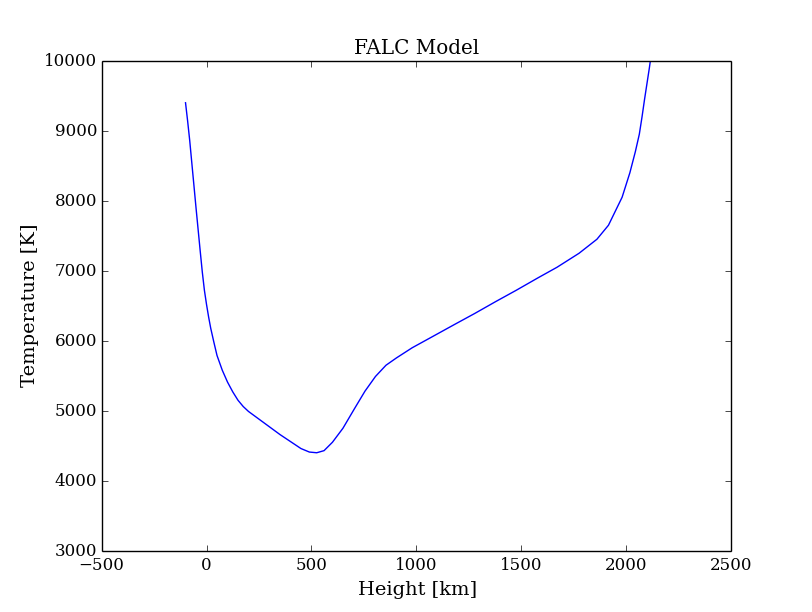
\includegraphics[width=.49\textwidth]{falctemp.png}
  \caption{Plot of temperature against column height.}
  \label{falctemp} 
 \end{figure}


\subsection{FALC density stratification}
I start by plotting the total pressure $p_{total}$ against colmn mass $m$. See figures \ref{falc_pressure} and \ref{falc_pressure_log}.
We see that they scale linearly. From this we can conclude that we can write 
\begin{equation}
 p_{total} = Cm
\end{equation}
where if one finds $C$ for all pressures and column masses and then find the average $C$, I get $C = g_{surface} = 27398.2$ cm/s$^2$.

\begin{figure}
 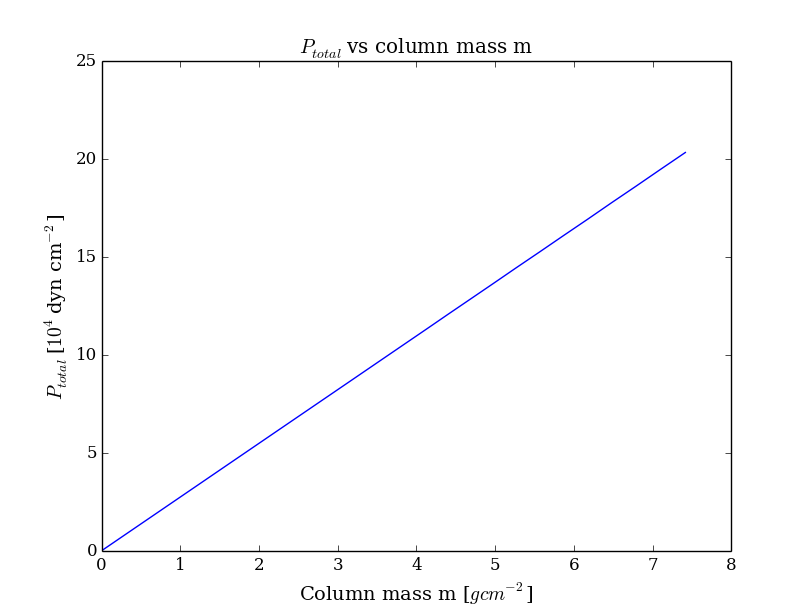
\includegraphics[width=.49\textwidth]{falc_pressure.png}
 \caption{Plot of total pressure against column mass.}
 \label{falc_pressure} 
\end{figure}
\begin{figure}
 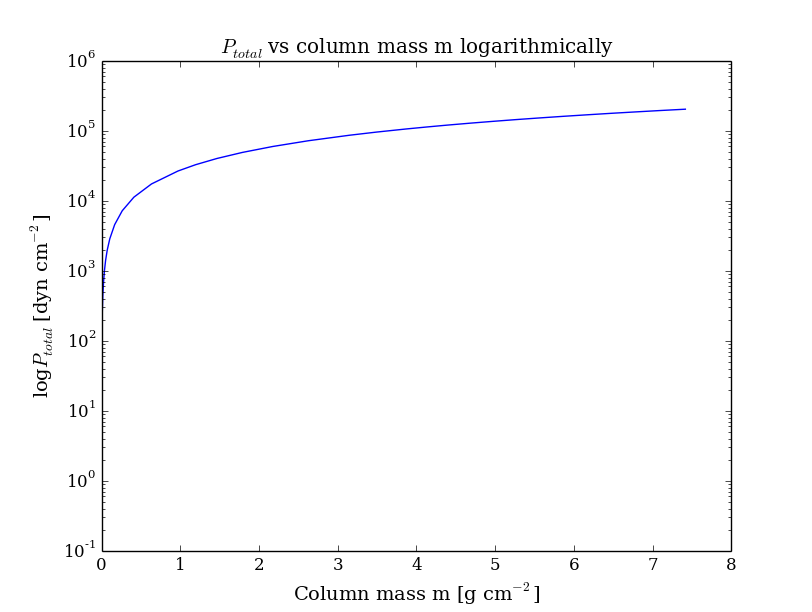
\includegraphics[width=.49\textwidth]{falc_pressure_log.png}
 \caption{Plot of total pressure against column mass using logarithmic scale.}
 \label{falc_pressure_log} 
\end{figure}

Fontena et a. (1993) assumed complete mixing, so we check that this condition holds by plotting the ratio of the hydrogen mass density to the total mass density against height. Next we add the Helium as well and calculate the contribution of helium and hydrogen to the total. From the figure it seems that nearly all of the density is contributed form hydrogen and helium. However if one does the calculation one finds that the average fraction of the remaining elements (the ``metals'') contributes $0.002$ ($0.02 \%$) of the total .This can be seen in figure \ref{Hdensratio_height}
\begin{figure}
 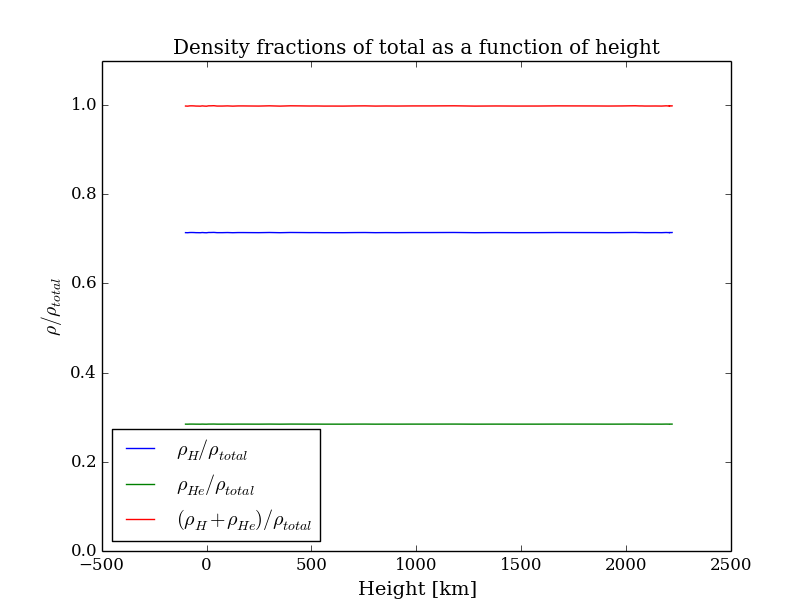
\includegraphics[width=.49\textwidth]{Hdensratio_height.png}
 \caption{Ratio of hydrogen mass density to total mass density vs height.}
 \label{Hdensratio_height} 
\end{figure}

Next we plot the column mass against height. See figure \ref{colm_height}. Note that the curve becomes nearly straight if we make the y-axis logarithmic in figure \ref{colm_height_log}. This is caused by XXXXXXXXXXXXXXXXXXXXXXXXX.
\begin{figure}
 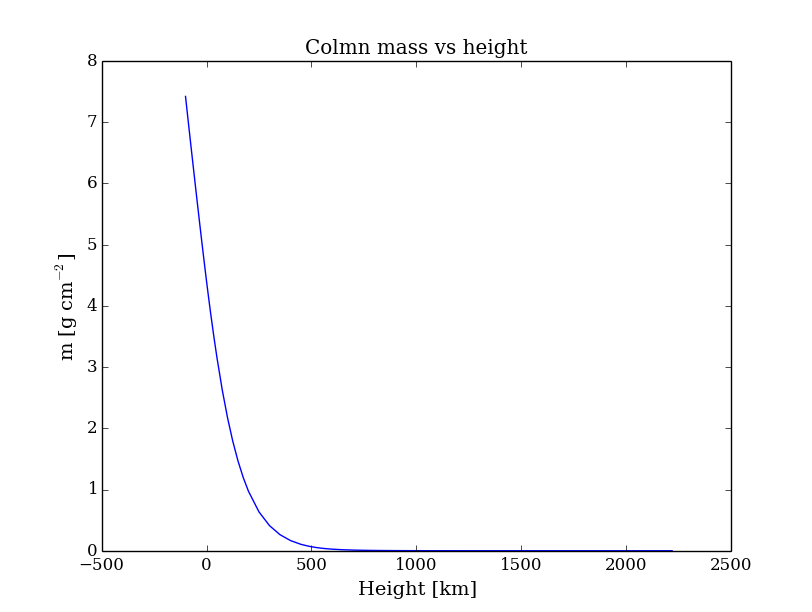
\includegraphics[width=.49\textwidth]{col_height.png}
 \caption{Column mass vs height.}
 \label{colm_height} 
\end{figure}

\begin{figure}
 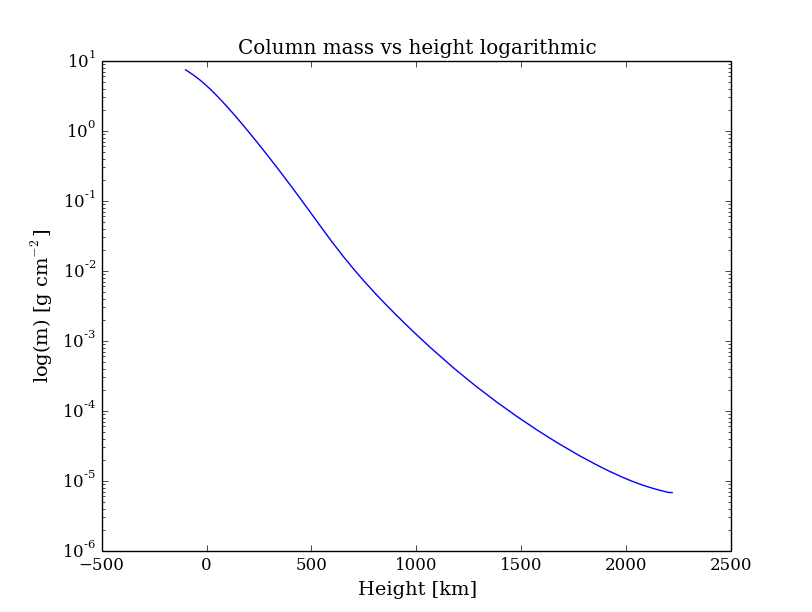
\includegraphics[width=.49\textwidth]{col_height_log.png}
 \caption{Column mass vs height with logarithimic y-axis.}
 \label{colm_height_log} 
\end{figure}

The next quantity to look at is gas density. Gas density is plotted against height in figure \ref{gdens_height}.

\begin{figure}
 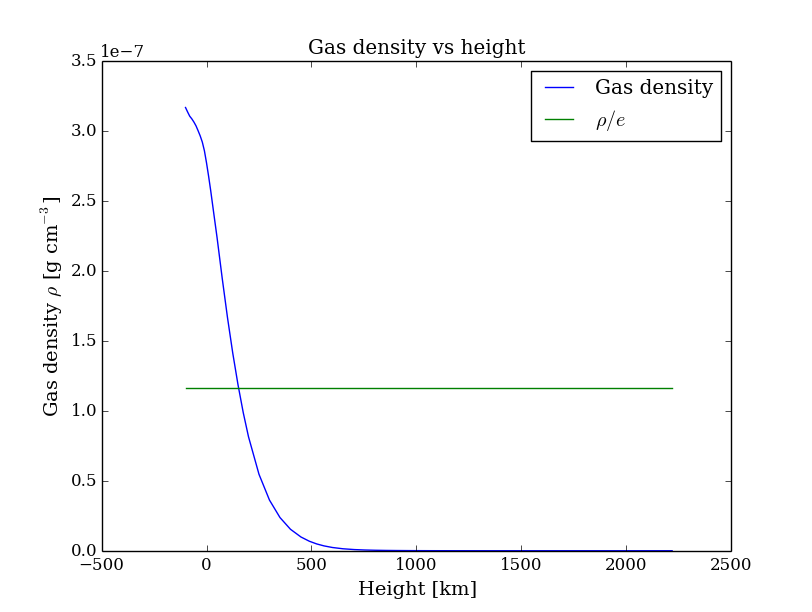
\includegraphics[width=.49\textwidth]{gdens_height.png}
 \caption{Gas density against height with the point where $\rho = \rho_0/e$ marked with a line.}
 \label{gdens_height} 
\end{figure}

We want to know the pressure scale height $H_\rho$ in  
\begin{equation}
 \rho \approx \rho(0)exp(-h/H_{\rho})
\end{equation}

This can be found from the definition
\begin{equation}
 H_\rho = \frac{kT}{M g}
\end{equation}
where $k$ is boltzmanns constant, T is temperature in K, M is the mean molecular weight, and g is surface gravity.
If one assumes that most of the molecules in the photosphere is hydrogen we can set $M=m_H$. Inserting the values for the deep photosphere ($h = -100$) then gives a scale height of $H_\rho = 196.3$ km. This is not realistic. Assuming that the photosphere only contains helium gives a scale height $H_\rho = 49.3 km$. The real number is somewhere between these two, but since we don't know the mean molecular weight this method doesn't really work in this case.

Another way to do this is to just mark the point where the density has fallen to $1/e$ of its original value. In figure \ref{gdens_height} this is marked with a line. The point the two lines cross gives $H_\rho \approx 150 $km.

The next step is to compute the gas pressure and plot it against height. We also overplot the product $(n_H + n_e)kT$. See figure \ref{gas_height}. There is some difference between the curves. Plotting the ratio between the curves shows this clearly (figure \ref{gas_height_ratio}). Note however that the sun does not only contain hydrogen. Because of this we must include the hydrogen number density in the ideal gas law. By doing this we obtain figure \ref{gas_height_hel} which shows a curve that seems to be overlapping perfectly. Plotting the ratio between the two curves shows that it deviates only slightly at the fourth decimal place. See figure \ref{gas_height_ratio_hel}. From this we can conclude that the ideal gas law is a very good approximation.

\begin{figure}
 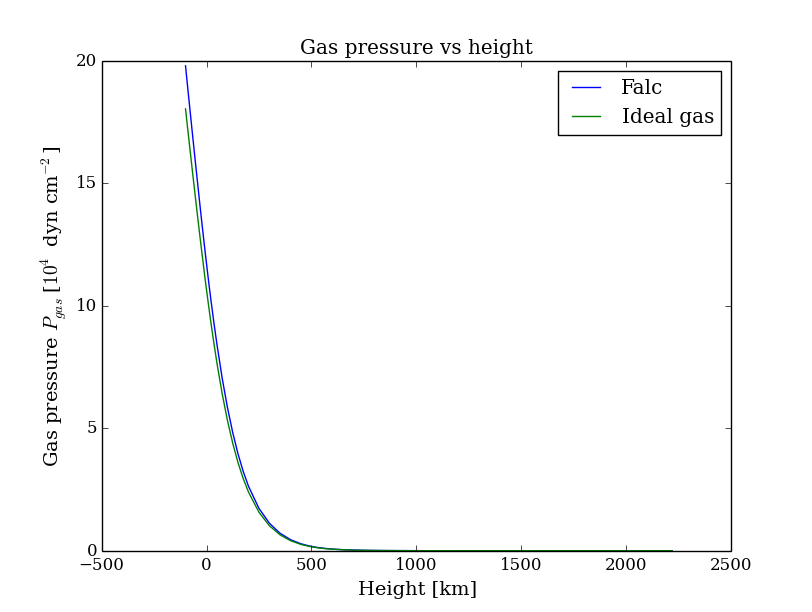
\includegraphics[width=.49\textwidth]{gas_height.png}
 \caption{Gas pressure against height.}
 \label{gas_height} 
\end{figure}

\begin{figure}
 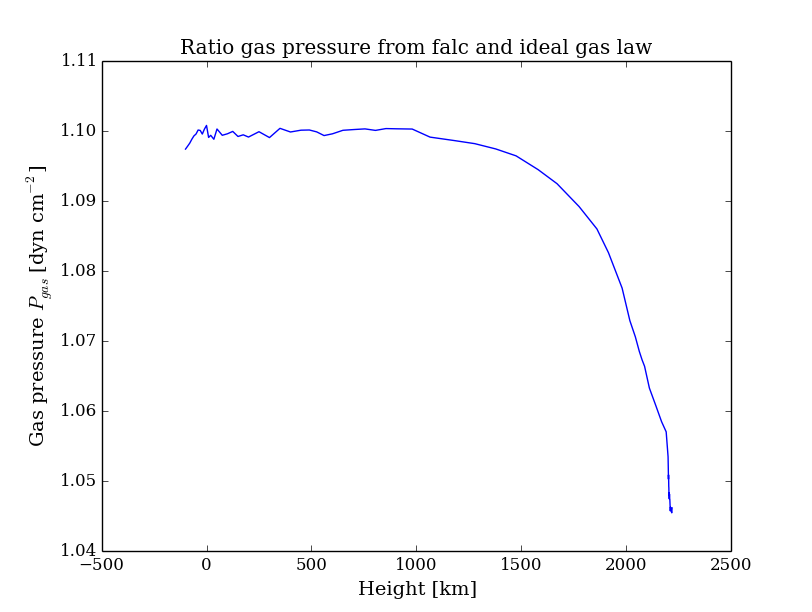
\includegraphics[width=.49\textwidth]{gas_height_ratio.png}
 \caption{Ratio between gas pressure and ideal gas law.}
 \label{gas_height_ratio} 
\end{figure}

\begin{figure}
 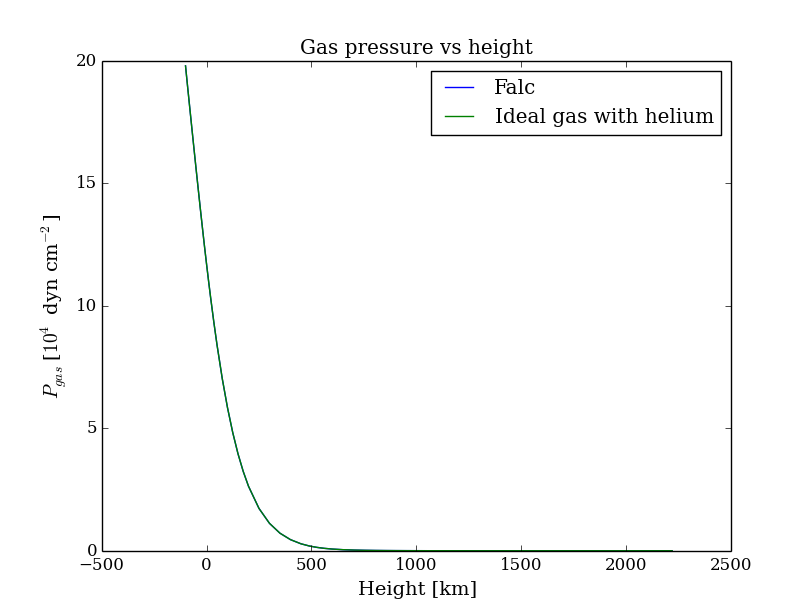
\includegraphics[width=.49\textwidth]{gas_height_hel.png}
 \caption{Gas pressure against height with helium included in curve forideal gas law.}
 \label{gas_height_hel} 
\end{figure}

\begin{figure}
 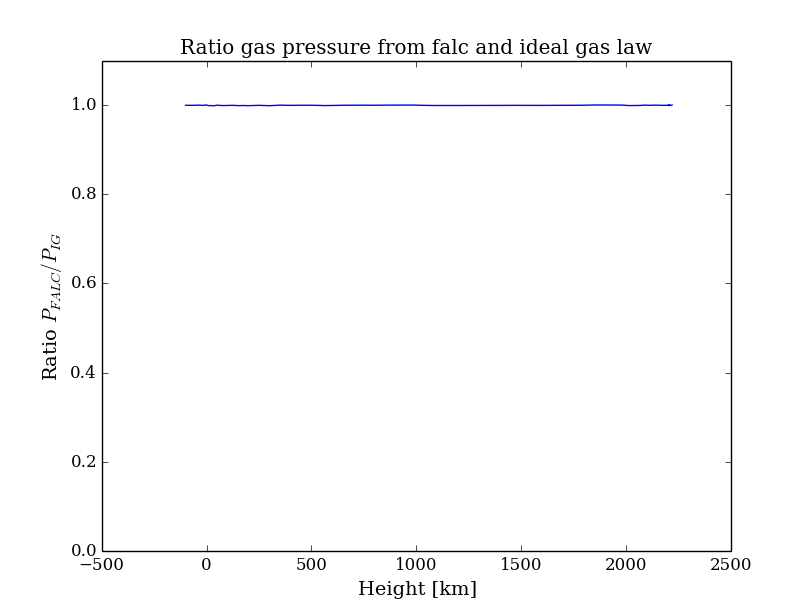
\includegraphics[width=.49\textwidth]{gas_height_ratio_hel.png}
 \caption{Ratio between gas pressure and ideal gas law when including helium.}
 \label{gas_height_ratio_hel} 
\end{figure}

With that done we want to look at the total hydrogen density. We should also include the electron density, proton density, and the density of the electrons that do not result from hydrogen ionization. The electron density, proton density and electron density can be read out of the FALC model. To find the density of the electrons not from ionized hydrogen we need to assume that all of the protons come from ionized hydrogen. This would indicate that $n_H - n_p$ equals the number of neutral hydrogen atoms. And since each neutral hydrogen has one electron this would be the number of electrons still bound to hydrogen, e.g those not from ionized hydrogen. The density of these should then be
\begin{equation}
 n_{be} = (n_H - n_p).
\end{equation}
This is plotted against height in figure \ref{densities_height}. 
\begin{figure}
 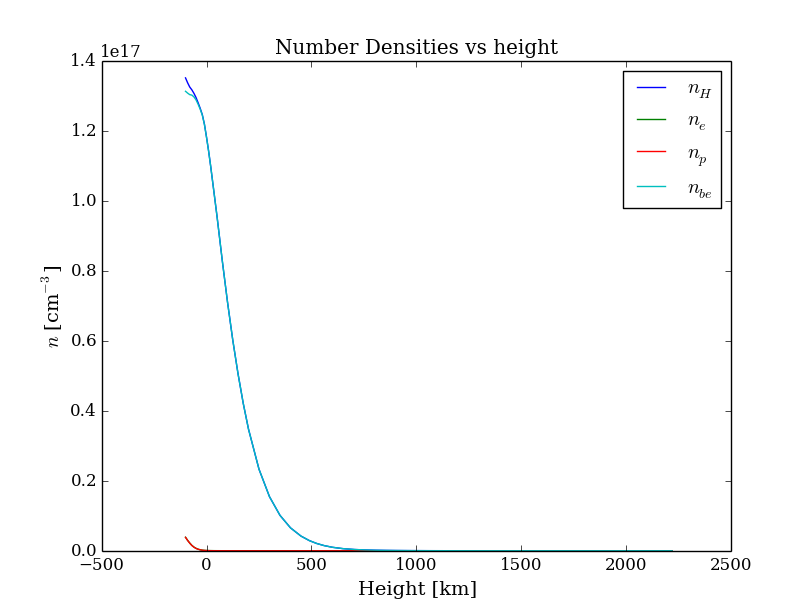
\includegraphics[width=.49\textwidth]{densities_height.png}
 \caption{Figure shows densities for a number of quantities against height.}
 \label{densities_height} 
\end{figure}

From the graph we see that the number density of protons is a little above 0 for very low heights. This indicates that the hydrogen gets ionized at this height. As the height increases this goes to zero indicating that the hydrogen remains neutral when height increases. Because of this it is only logical that the electron density goes to zero as well, and that the density of the elctrons not from ionized hydrogen approaches the density of the hydrogen (since nearly all of the hydrogen is neutral hydrogen). Figure \ref{densities_height_log} shows the same with a logarithmic
\begin{figure}
 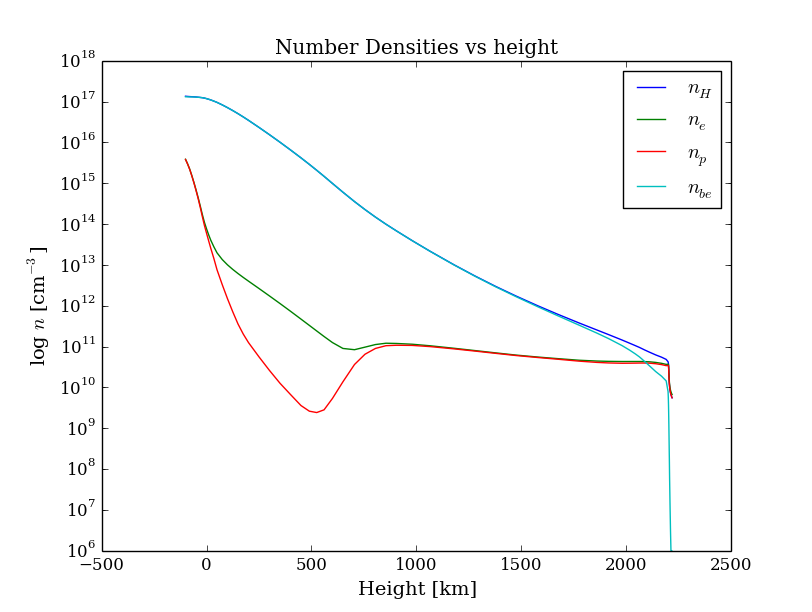
\includegraphics[width=.49\textwidth]{densities_height_log.png}
 \caption{Figure shows densities for a number of quantities against height with logarithmic y-axis.}
 \label{densities_height_log} 
\end{figure}

As the height increases the number density of everything approaches zero, which makes sense since we are looking at the atmosphere of the sun. At some point we should approach vacuum which has almost zero density.

With that done we plot the ionization fraction of hydrogen against height. 
The ionization fraction of hydrogen fraction is simply
\begin{equation}
 n_{HII} = \frac{n_p}{n_H}
\end{equation}

See figure \ref{hyd_ion}. Note the logarithmic scale.
\begin{figure}
 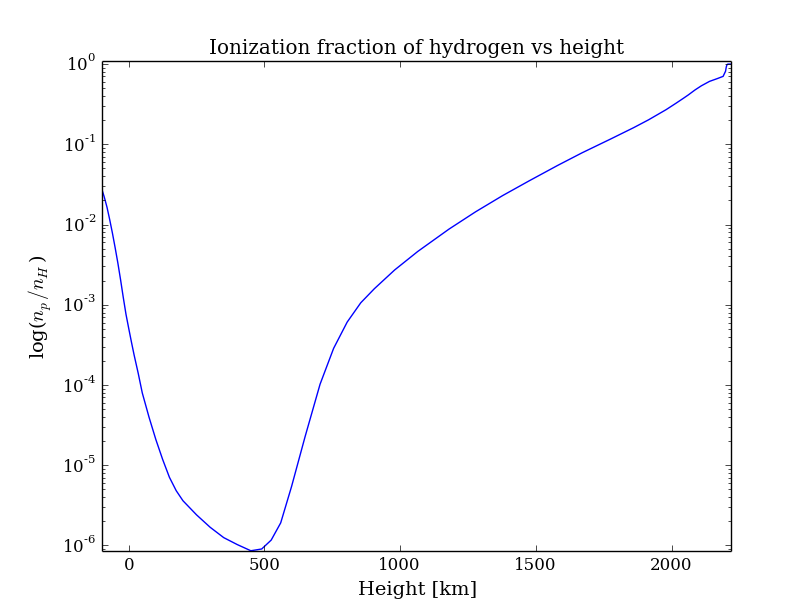
\includegraphics[width=.49\textwidth]{hyd_ion.png}
 \caption{Figure shows the ionization fraction of hydrogen depending on height in kilometers.}
 \label{hyd_ion} 
\end{figure}
There is a clear resemblence to the temperature plot (see figure \ref{falctemp}).
XXXXXXXXXXXXXXXXXXXXXXXXX EXPLAIN WHY THAT IS AND WHY IT IS TILTED XXXXXXXXXXXXXXXXXXXXXXXXX



The next thing one should do is compare the photon density to the particle density.
If one assumes thermodynamic equilibrium the photon density $N_{phot}$ in photons per cm$^3$ is given by
\begin{equation}
 N_{phot} \approx 20T^3
\end{equation}

XXXXXXXXXXXXXXXXXXXXXXXXX EXPLAIN WHY THIS IS XXXXXXXXXXXXXXXXXXXXXXXXX.
Calculating this value for the deep photosphere ($h = -100$) gives a photon density $N_{phot} = 1.66\times10^{13}$ cm$^{-3}$. In comparison the hydrogen density at the same location is $N_H = 1.35\times10^{17}$ cm$^{-3}$. 
Unfortunately we can not assume thermodynamic equilibrium higher up in the atmosphere. The equation for the photon density there instead becomes
\begin{equation}
 N_{phot} = 20T_{eff}^3/2\pi
\end{equation}
where $T_{eff} = 5770$K is the effective solar temperature.
Calculating this for the highest point in our data gives $N_{phot} = 6.11\times 10^{11}$ cm$^{-3}$. The density of hydrogen a
t the same point is $N_H = 5.58\times 10^9$. At this height there are more photons than hydrogen atoms. Note that the hydrogen density dropped by 8 orders of magnitude, while the photon density dropped only 2.
The medium at this high altitude is insensitive to the photons because XXXXXXXXXXXXXXXXXXXXXXXXX EXPLAIN WHY XXXXXXXXXXXXXXXXXXXXXXXXX.

\subsection{Comparison with the earth's atmosphere}
There have been done similar measurements of the earths atmosphere. The values used in this report are from Allen 1976. 
The first thing to do is to make plots of everything in the table. See figures \ref{temp_earth}, \ref{pressure_earth}, \ref{particle_dens_earth}, and \ref{gas_dens_earth}.

\begin{figure}
 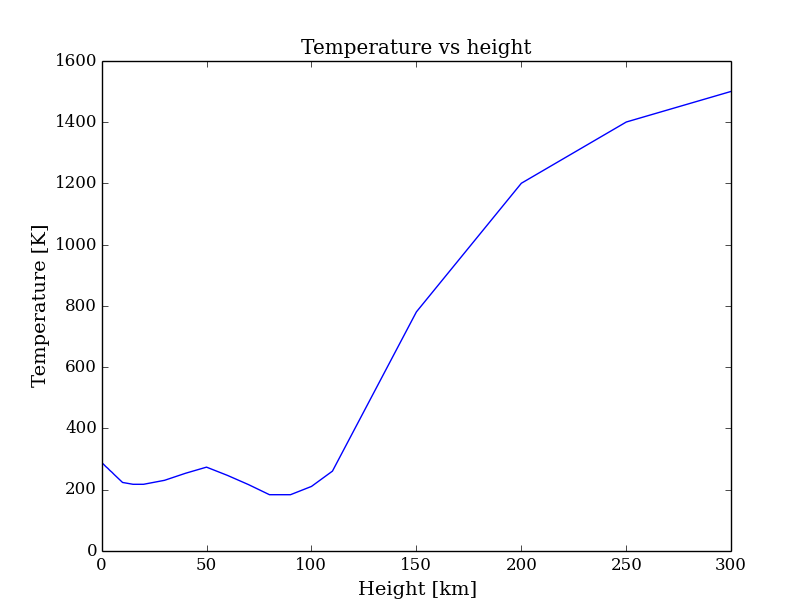
\includegraphics[width=.49\textwidth]{temp_earth.png}
 \caption{Plot of the temperature as a function of height above the surface on earth.}
 \label{temp_earth} 
\end{figure}

\begin{figure}
 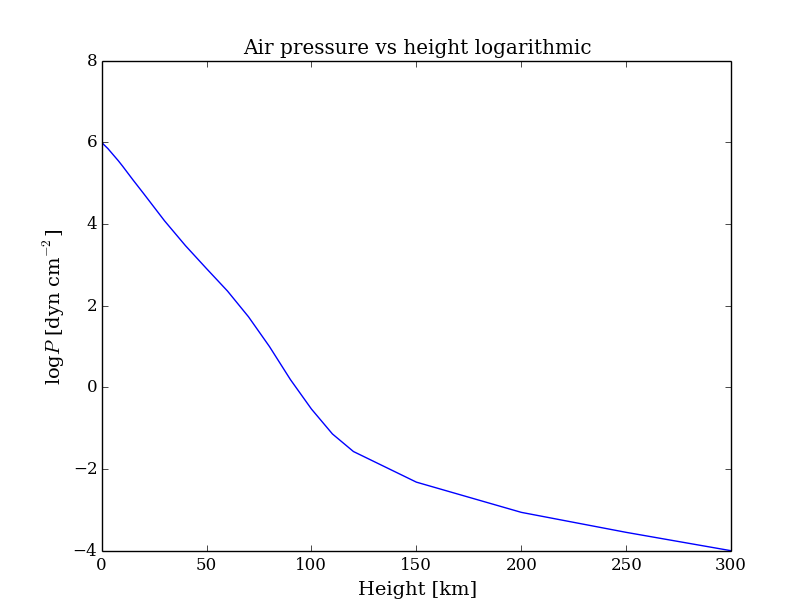
\includegraphics[width=.49\textwidth]{pressure_earth.png}
 \caption{The figures shows the pressure as function of height on earth.}
 \label{pressure_earth} 
\end{figure}

\begin{figure}
 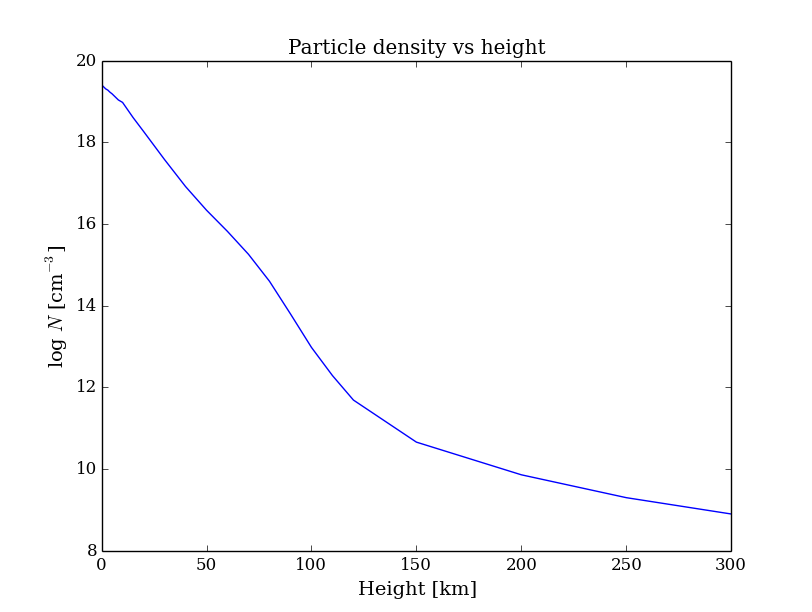
\includegraphics[width=.49\textwidth]{particle_dens_earth.png}
 \caption{Particle density against height.}
 \label{particle_dens_earth} 
\end{figure}

\begin{figure}
 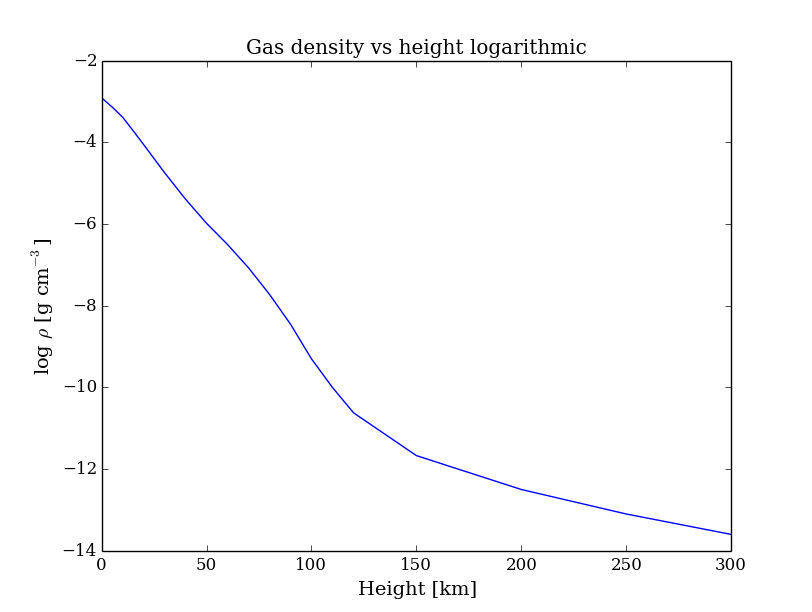
\includegraphics[width=.49\textwidth]{gas_dens_earth.png}
 \caption{Plot of the gas density as a function of height on earth.}
 \label{gas_dens_earth} 
\end{figure}

Taking a closer look at pressure and density reveals that if one normalizes each to their respective maximums and then plot them together we get a graph that is very close to identical.
XXXXXXXXXXXXXXXXXXXXXXXXX COMMENT WHY THEY LOOK THE SAME XXXXXXXXXXXXXXXXXXXXXXXXX

Next we plot the mean molecular weight $\mu_E \equiv \overline{m}/m_H$ against height. See figure \ref{mu_E}. We see that it decreases at higher altitudes. This is caused by XXXXXXXXXXXXXXXXXXXXXXXXX EXPLAIN WHY XXXXXXXXXXXXXXXXXXXXXXXXX.
\begin{figure}
 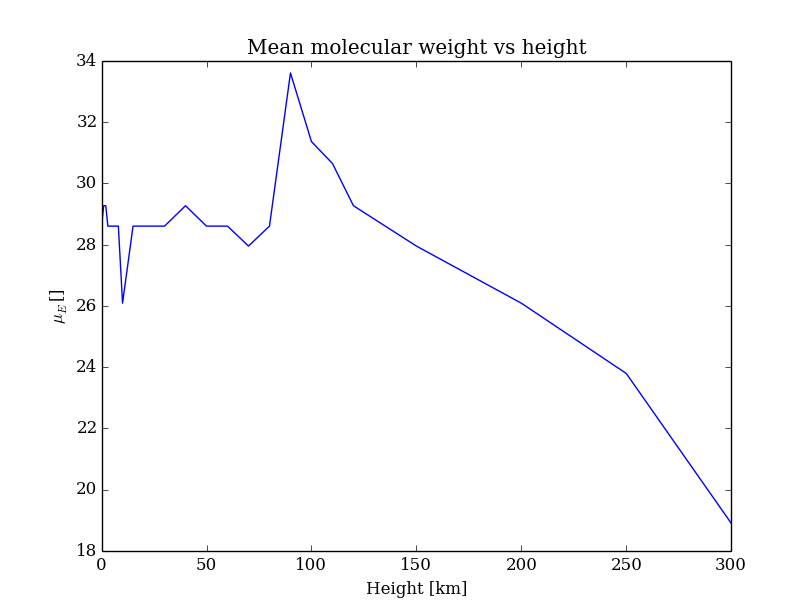
\includegraphics[width=.49\textwidth]{mu_E.png}
 \caption{Mean molecular weight versus height on earth.}
 \label{mu_E} 
\end{figure}

We should also se what the density scale height is in the lower atmosphere. Like for the sun we can do this two different ways. Either by using the equation for the scale height
\begin{equation}
 H_\rho = \frac{kT}{Mg}
\end{equation}
where everything means the same as before. The difference is that in this case we actually know the mean molecular weight. Inserting values gives $H_\rho = 8.54$ km at the surface of earth. Approximating with the same method as earlier gives $H_\rho \approx 9.5$ km. In this case I would trust the first one more since we know the values we use in the equation to a good precision. Note that the scale height on earth is more than 10 times smaller than on the sun. This is of course caused by the large difference in surface gravity and temperature.

Comparing the rest of the quantities for the sun and earth at the surface shows many differences.
\begin{table}
\begin{tabular}{|c|c|c|}
\hline
&Sun & Earth\\
\hline
$\rho$ &$2.77\times 10^{-7}$g cm$^{-3}$ &$1.23\times 10^{-3}$g cm$^{-3}$\\
\hline
N &$1.30\times10^{17}$cm$^{-3}$ &$2.57\times10^{19}$cm$^{-3}$ \\
\hline
P &$1.21\times10^{5}$dyn cm$^{-3}$ &$1.02\times10^{6}$dyn cm$^{-3}$ \\
\hline
T &$6520$K &$288$K\\
\hline
\end{tabular}
\caption{Table with different values for the earth and the sun}
\end{table}
Note especially that the ratio between particle density at the surface of earth to the surface of the sun is almost 200.

If we now calculate the column mass for the surface of earth we find that it is $1044$g cm$^{-2}$. For the sun the column mass on the surface was $4.404$g cm$^{-2}$.

If we now calculate the photon density reaching earth from the sun
\begin{equation}
 N_{phot} = \pi \frac{R^2}{D^2}N_{phot}^{top}
\end{equation}
where $N_{phot}^{top}$ is the photon density we found earlier at the top of the solar atmosphere, we find that $N_{phot} = 4.16\times10^{7}$cm$^{-3}$ reaching us from the sun.
While if we calculate the thermal photon density from the earth atmosphere we get $N_{phot}^{earth} = 4.78\times 10^8$cm$^{-3}$. Which means that there are more than 10 times more photons coming from the earth atmosphere on the surface of earth than we receive from the sun. Calculating the ratio of the received photons and the particle density in the air gives a ratio of $1.6\times 10^{-12}$. So the photon density is smaller by 12 orders of magnitude.

XXXXXXXXXXXXXXXXXXXXXXXXX COMMENT XXXXXXXXXXXXXXXXXXXXXXXXX.

\section{Continous spectrum from the solar atmosphere}
In this section we want to look at the formation of the solar continuum. We concentrate on the visible and near-infrared parts of the spectrum.
\subsection{Observed solar continua}
We will be using the table provided by Allen (1976) for this part. It specifies the continuum radiation emitted by the sun in the wavelength range $\lambda = 0.2 - 5\mu$m. This table specifies four different quantities as a function of wavelength. The quantites are radially emergent intensity and the astrophysical flux in the solar continuum with, and without, smoothed lines.

The four quantites are plotted in figure \ref{distrib}.
\begin{figure}
 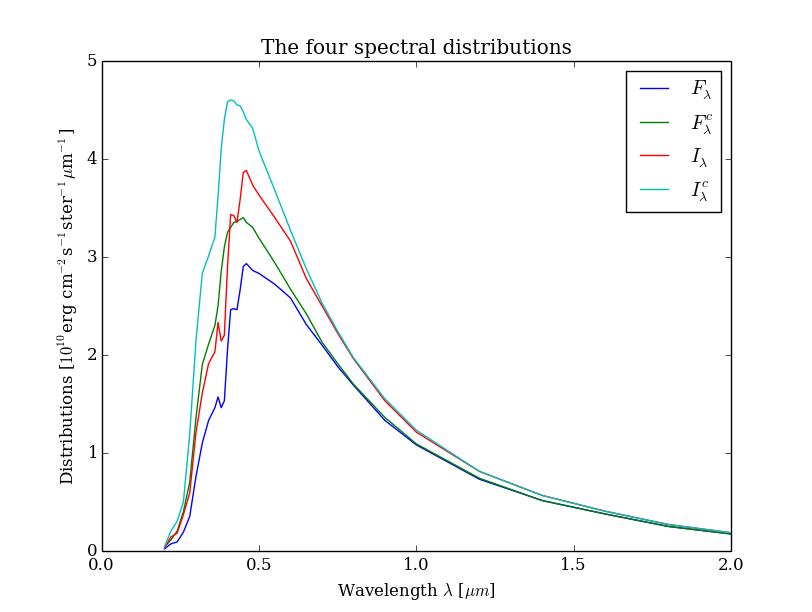
\includegraphics[width=.49\textwidth]{distrib.png}
 \caption{The four disitributions.}
 \label{distrib} 
\end{figure}
XXXXXXXXXXXXXXXXXXXXXXXXX EXPLAIN WHY THEY SHARE THE SAME UNITS AND THEIR DIFFERENCES   XXXXXXXXXXXXXXXXXXXXXXXXX

Next we convert the distributions into values per frequency bandwitch $\Delta \nu = 1$ Hz, and plot them against wavelength. (See figure \ref{distrib_freq}).
\begin{figure}
 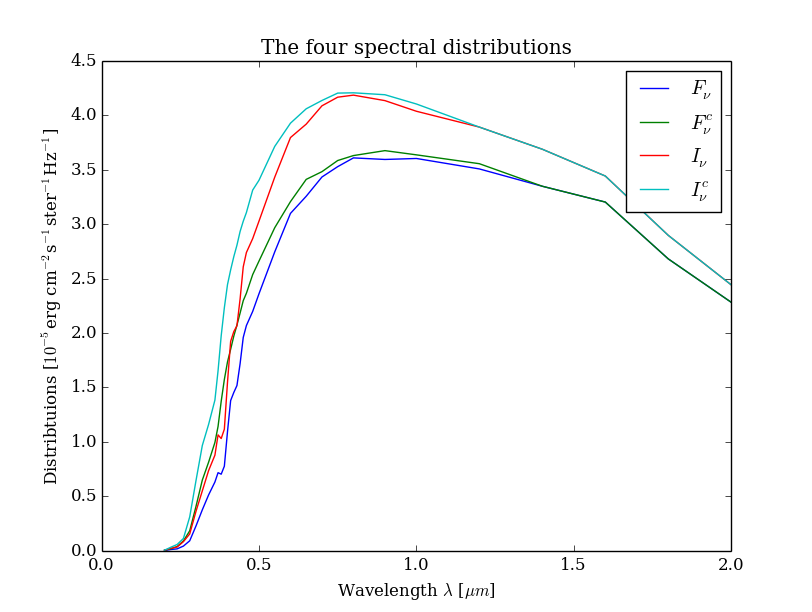
\includegraphics[width=.49\textwidth]{distrib_freq.png}
 \caption{The four disitributions converted to frequency.}
 \label{distrib_freq} 
\end{figure}

We should try to approximate the intensity of the continuum with a planck fit.
Figure \ref{planckfit} has the planck function with 3 different tempetatures in the same plot as the solar continuum intensity. 
\begin{figure}
 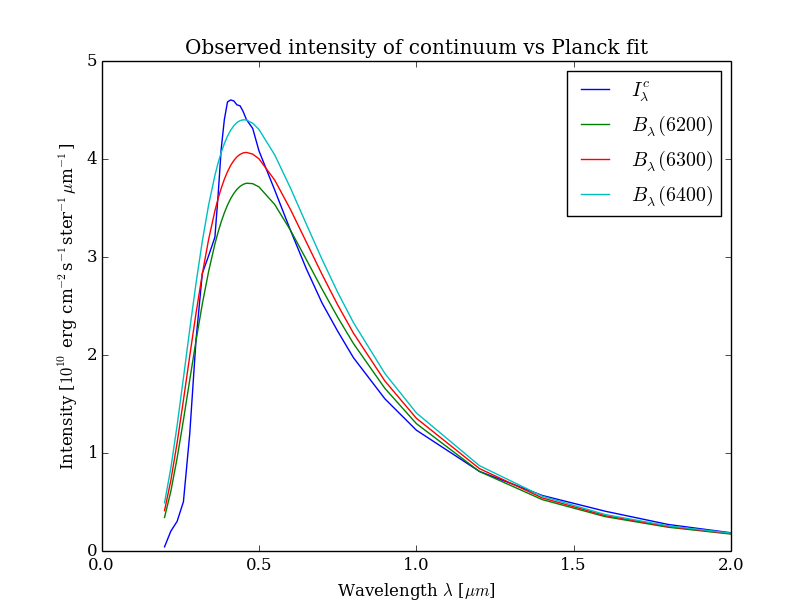
\includegraphics[width=.49\textwidth]{planckfit.png}
 \caption{The solar continuum with three attempts to fit a planck function to it.}
 \label{planckfit} 
\end{figure}
The same can also be done for the ones converted to frequency (See figure \ref{planckfit_freq}).
\begin{figure}
 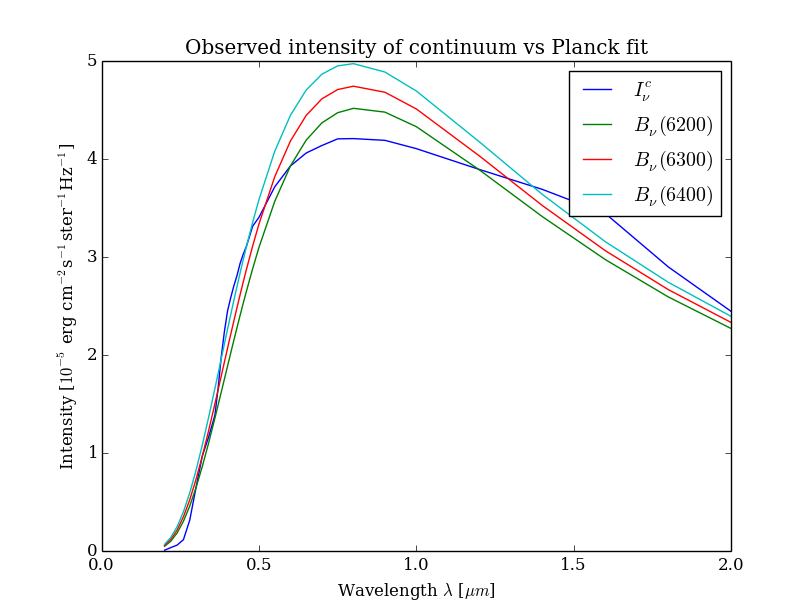
\includegraphics[width=.49\textwidth]{planckfit_freq.png}
 \caption{The solar continuum with three attempts to fit a planck function to it.}
 \label{planckfit_freq} 
\end{figure}
Comparing the two it is clear that something in the range 6200-6400 K is as good as we will get. I will go with 6300 K.


Inverting the planck function and inserting the solar continuum produces figure \ref{planck_invert}
\begin{figure}
 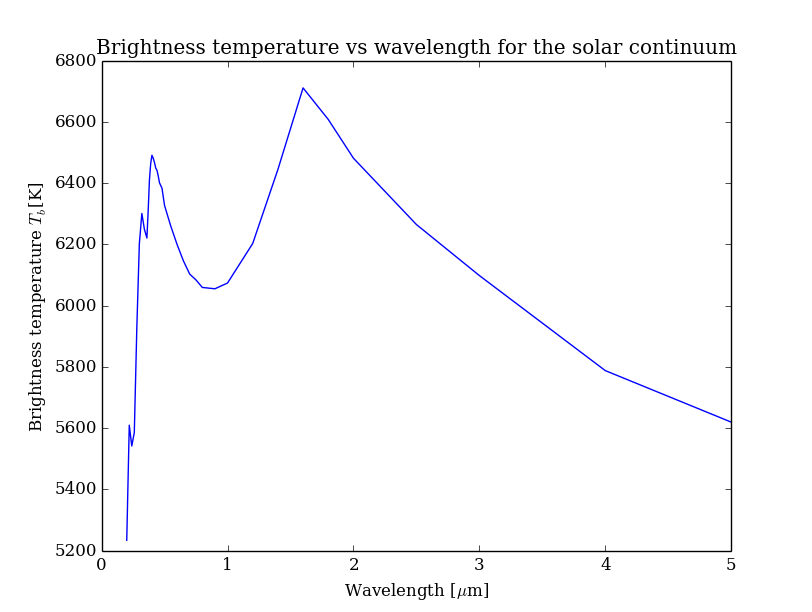
\includegraphics[width=.49\textwidth]{planck_invert.png}
 \caption{Brightness temperature of the solar continuum.}
 \label{planck_invert} 
\end{figure}
We see that it peaks at $\lambda \approx 1.6 \mu$m.
This is in the short-wavelength infrared region of the spectrum. There is also a peak around $0.4 \mu$m. This corresponds to violet in the visual spectrum. So in other words; the light we see receieve from the sun should be slightly more violet in color than the others. Whether increasing the brightness temperature from 6100K to 6500K results in something we can actually see is another question (Note that this could not be seen while inside the earth atmosphere because scattering changes the spectrum one receives considerably). Nevertheless the peak in the infrared region is even higher than the violet one. That peak is also a wider one which would indicate that more energy is transported through infrared radiation than visible light.
\subsection{Continuous extinction}
Now we aim to reproduce figure 5 in the project text. We are provided with a function that evaluates polynomial fits for H$^-$ extiction that are given on page 135 ff of Gray (1992). This function delivers the total H$^-$ extinction in units of cm$^2$ per neutral hydrogen atom. Plotting the values corresponding to the electron density and temperature at the surface of the solar atmosphere results in figure \ref{extinction}. The function works as it should, and we get a nice curve corresponding with Gray's version in the project text.
\begin{figure}
 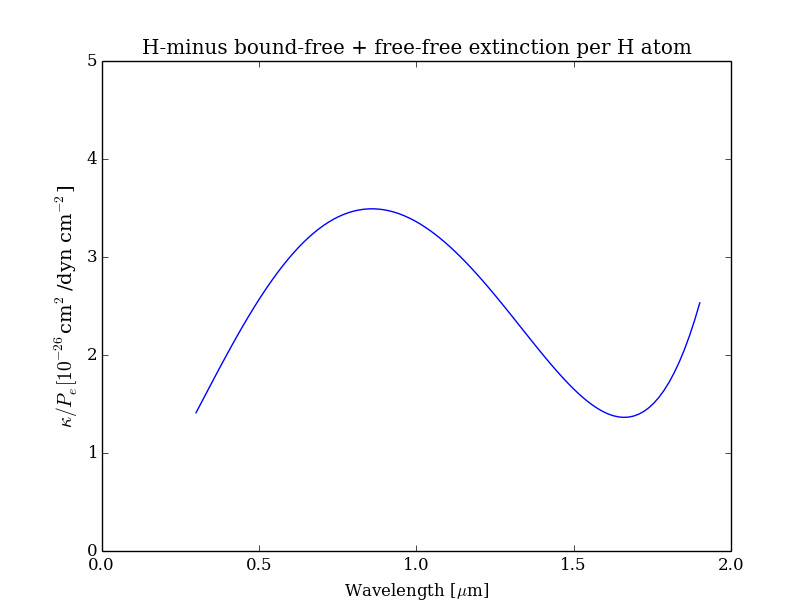
\includegraphics[width=.49\textwidth]{extinction.png}
 \caption{H$^-$ extinction for FALC parameters at surface of solar atmosphere, normalized with the electron pressure $P_e =n_e kT$.}
 \label{extinction} 
\end{figure}
Note that the H$^-$ extinction is not hydrogenic, this is caused by XXXXXXXXXXXXXXXXXXXXXXXXX EXPLAIN XXXXXXXXXXXXXXXXXXXXXXXXX.

We can actually make this resemble the plot for brightness temperature against wavelength by XXXXXXXXXXXXXXXXXXXXXXXXX EXPLAIN WHAT YOU DO  AND WHY IT WORKS XXXXXXXXXXXXXXXXXXXXXXXXX.

It would be interesting to study how the extinction behaves at different hights.
To do this we use the values from the FALC model, and look at insert values corresponding to every height in the data at $\lambda = 0.5 \mu$m.  Note that the units have changed since the last plot. This is because we are now looking at extinction $\alpha_\lambda(H^-)$ measured per cm path length instead of per H atom. To get this we multiplied the result obtained from the function creating polynomial fits with the number density of neutral hydrogen atoms $n_{neutral H} \approx n_H(h) - n_p(h)$. Note that the y-axis is on a log scale so that one can see the behaviour of the function. It would also be useful to include the extinction due to free electrons. The extinction due to free electrons should simply be $\alpha_e = \sigma^T n_e$, where $\sigma^T = 6.648\times 10^{-25}$cm$^2$ i the thomson cross-section, and $n_e$ is the number density of electrons. 
The results can be seen in figure \ref{extinc_5000}.

\begin{figure}
 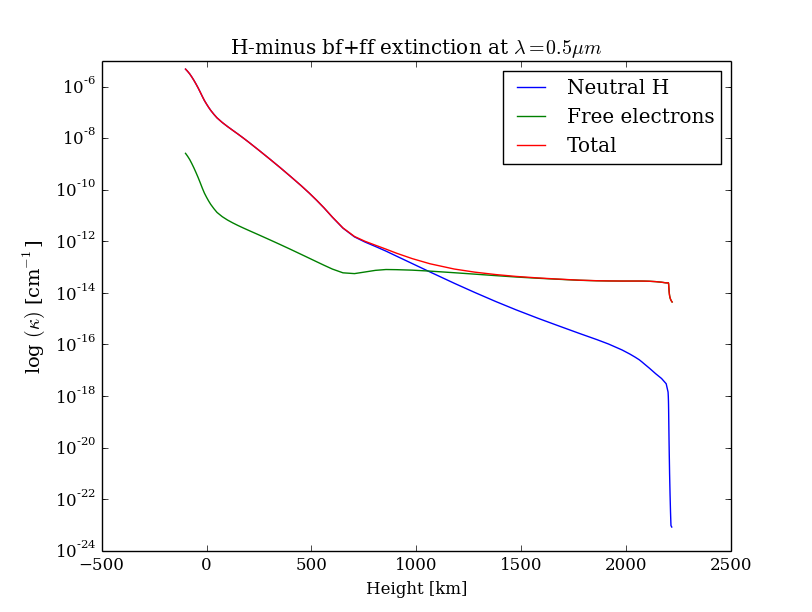
\includegraphics[width=.49\textwidth]{extinc_5000.png}
 \caption{H$^-$ extinction for FALC parameters for $\lambda = 0.5\mu$m in solar atmosphere per centimeter path length.}
 \label{extinc_5000} 
\end{figure}
We see in the figure that extinction from neutral hydrogen dominates for low heights, but as we increase the height the number density of hydrogen decreases, causing a decrease in the extinction from the neutral hydrogen. We also note that the number density of electrons also decreases, but it does not fall as steeply, and when we reach about 850 km it remains constant up until 2200 km. The neutral hydrogen keeps decreasing. This is caused by a combination of hydrogen number density decreasing as well as ionization at higher altitudes. 

\subsection{Optical Depth}
Knowing the stratification from the FALC model, and the continous extinction allows us to compute the otical depth given by 
\begin{equation}
 \tau_\lambda(h_0) \equiv - \int_\infty^{h_0}\alpha_\lambda^c dh
\end{equation}
I use trapezoidal integration to calculate this and compare it to the one tabulated in the FALC data. See figure \ref{optical_depth}.
\begin{figure}
 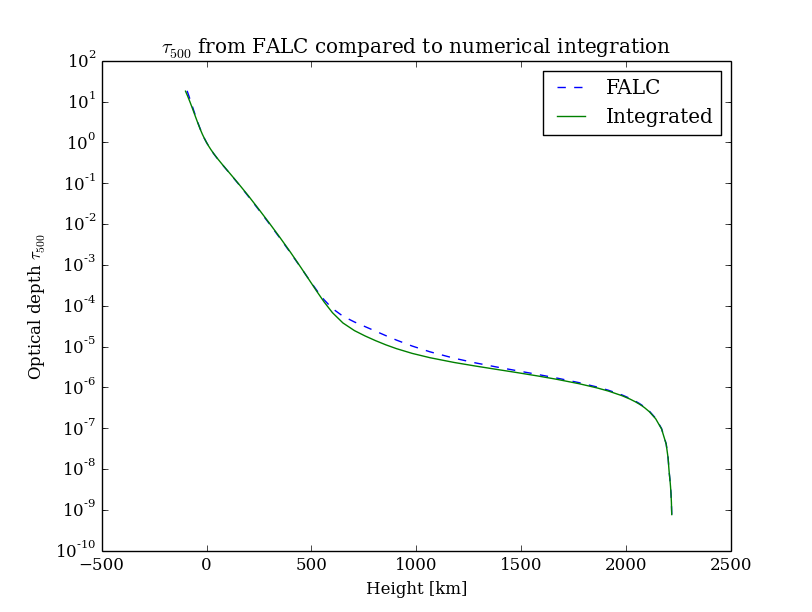
\includegraphics[width=.49\textwidth]{optical_depth.png}
 \caption{Optical depth $\tau_{500}$ from the FALC model compared to the one calculated using polynomial fits.}
 \label{optical_depth}
\end{figure}
The two correspond very well. There is however a gap separating the two which is not unexpected considering how few points we are integrating over.
\subsection{Emergent intensity and height of formation}
If one assumes plane-parallell stratification, the emergent intensity from the solar disk can be written
\begin{equation}
 I_\lambda = \int_0^\infty S_\lambda e^{-\tau_\lambda}d\tau_\lambda.
\end{equation}
We should also inspect the intensity contribution function
\begin{equation}
 \frac{dI_\lambda}{dh} = S_\lambda e^{-\tau_\lambda}\alpha_\lambda.
\end{equation}
This function gives contribution of each layer at a height h to the emergent intensity. Its weighted mean defines the ``mean height of formation'' and is given by
\begin{equation}
 <h> = \frac{\int_0^\infty h(dI_\lambda/dh)dh}{\int_0^\infty(dI_\lambda/dh)dh} = \frac{\int_0^\infty hS_\lambda e^{-\tau_\lambda}d\tau_\lambda}{\int_0^\infty S_\lambda e^{-\tau_\lambda}d\tau_\lambda}
\end{equation}

We use trapezoidal integration to compute the integral. Obviously we dont have an infinite number of optical depths to integrate over so this will not be an exact solution but it should still give a result very close to the real one.

We choose to look at $\lambda  = 5000 \AA$ ($0.5\mu$m). The computation results in an intensity $4.29\times10^{10}$erg cm$^{-2}$s$^{-1}\mu$m$^{-1}$ster$^{-1}$. The observed intensity at this wavelength is $4.08\times10^{10}$erg cm$^{-2}$s$^{-1}\mu$m$^{-1}$ster$^{-1}$. We see a 4.87$\%$ deviation from the observed intensity, so the computation is good, considering the scales we are operating on.

Next we should plot the peak contribution function and compare it to the mean height of formation.
See figure \ref{contfunc_5000} for the plot. The peak for the normalized contribution function appears at height -30.0 km, while the mean height for formation is at -3.14 km.

\begin{figure}
 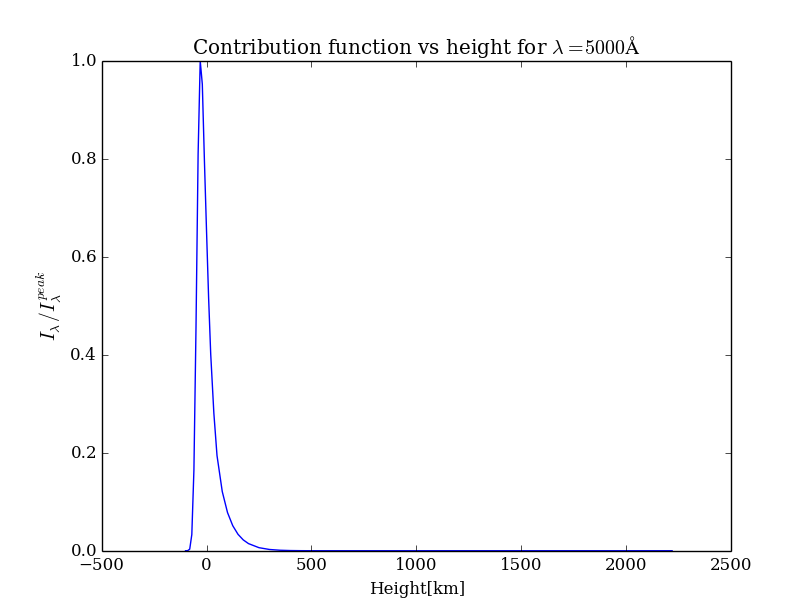
\includegraphics[width=.49\textwidth]{contfunc_5000.png}
 \caption{The contribution function for the intensity at $\lambda= 5000\AA$.}
 \label{contfunc_5000}
\end{figure}

Next we should study other wavelengths. At $\lambda = 10000\AA$ we get figure \ref{contfunc_10000}. Here the peak is at -20.0 km, while the mean height for formation is at 24.1 km.

\begin{figure}
 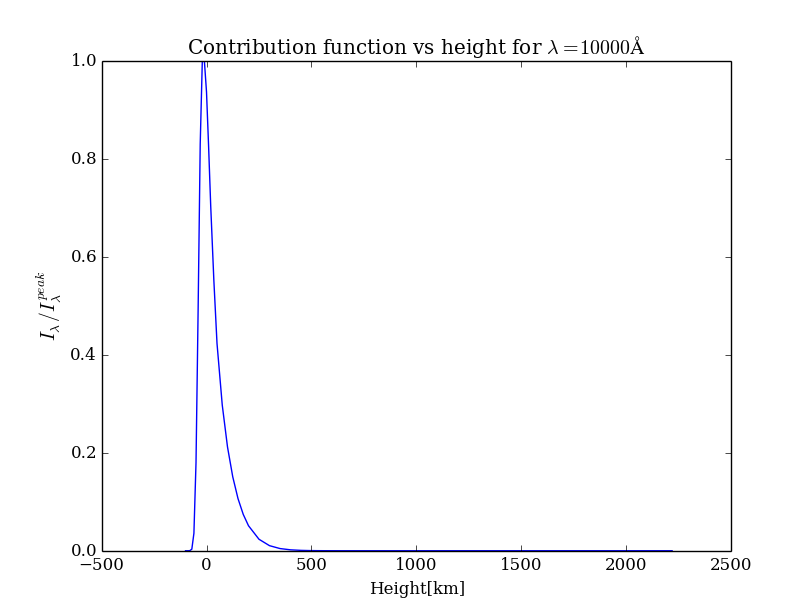
\includegraphics[width=.49\textwidth]{contfunc_10000.png}
 \caption{The contribution function for the intensity at $\lambda= 10000\AA$.}
 \label{contfunc_10000}
\end{figure}

Continuing to $\lambda = 16000\AA$ we get the peak at -30.0 km, and the mean height of formation at -17.9 km. See figure \ref{contfunc_16000}

\begin{figure}
 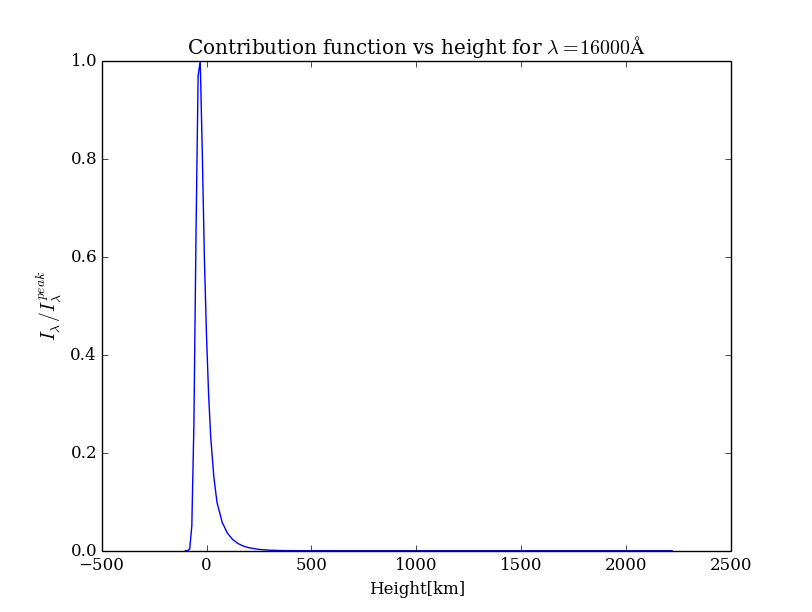
\includegraphics[width=.49\textwidth]{contfunc_16000.png}
 \caption{The contribution function for the intensity at $\lambda= 16000\AA$.}
 \label{contfunc_16000}
\end{figure}

At $\lambda = 50000\AA$ we se a huge drop in the intensity. (Note the change in units on the y-axis in figure \ref{contfunc_50000}). The peak shifts to 490.0 km. And the mean height shifts to 499.2 km.

\begin{figure}
 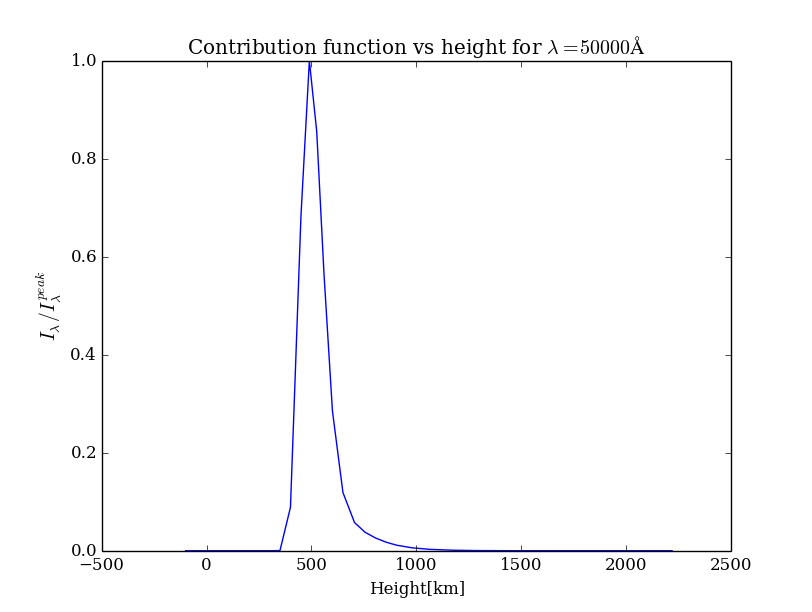
\includegraphics[width=.49\textwidth]{contfunc_50000.png}
 \caption{The contribution function for the intensity at $\lambda= 50000\AA$.}
 \label{contfunc_50000}
\end{figure}


The location of the peak shifts for the wavelengths, but its stays around the same height for the 3 first wavelengths. However if we switch to $\lambda = 50000 \AA$ it shoots up by several hundred kilometers. This can be attributed to XXXXXXXXXXXXXXXXXXXXXXXXX EXPLAIN WHY THE FUNCTION CHANGES XXXXXXXXXXXXXXXXXXXXXXXXX

We should also check the validity of the LTE Eddington-Barbier approximation. This is done by comparing the mean height of formation with the locations where $\tau_\lambda = 1$ and with the locations where $T_b = T(h)$.
Table \ref{ebtable} shows the values for the different wavelengths. While $h(\tau=1)$ and $<h>$ share some resemblence, $h_T$ is nowhere near any of them.

\begin{table}
\begin{tabular}{|c|c|c|c|}
\hline
$\lambda$&$h(\tau = 1)$ & $h_T$ &$<h>$ \\
\hline
$500$nm& $0.0$km &$10$km & $-3.1$km\\
\hline
$1000$nm&$10$km& $1065$km & $24.1$km\\
\hline
$1600$nm&$-30$km & $1476$km &$-17.9$km\\
\hline
$5000$nm&$490$km & $855$km & $499.2$km\\
\hline
\end{tabular}
\caption{Table shows the height where $\tau_\lambda = 1$, the height where $T_b = T(h)$, and the mean height of formation $<h>$. Note however that we do not have enough precision to find any points where $T_b$ is exactly equal to $T(h)$ so I have chosen to use the heights where the two are closest. Even so the deviations are at most 34K, and the lowest temperature is 5620K, which makes this deviation neglibible.}
\label{ebtable}
\end{table}



%\begin{acknowledgements}
%\end{acknowledgements}

%%%%%%%%%%%%%%%%%%%%%%%%%%%%%%%%%%%%%%%%%%%%%%%%%%%%%%%%%%%%%%%%%%%%%%%%%%%%
%% references
\section{References}
Rutten, R. J.: 1991, The Generation and Transport of Radiation, Sterrekundig Instituut Utrecht, The Netherlands

%\bibliographystyle{aa-note} %% aa.bst but adding links and notes to references
%\raggedright              %% only for adsaa with dvips, not for pdflatex
%\bibliography{XXX}          %% XXX.bib = your Bibtex entries copied from ADS

\end{document}


